\documentclass[a4paper,12pt]{article}
\usepackage[top = 2.5cm, bottom = 2.5cm, left = 2.5cm, right = 2.5cm]{geometry}
\usepackage[T1]{fontenc}
\usepackage[utf8]{inputenc}
\usepackage{multirow} 
\usepackage{booktabs} 
\usepackage{graphicx}
\usepackage[spanish]{babel}
\usepackage{setspace}
\setlength{\parindent}{0in}
\usepackage{float}
\usepackage{fancyhdr}
\usepackage{amsmath}
\usepackage{amssymb}
\usepackage{amsthm}
\usepackage[numbers]{natbib}
\newcommand\Mycite[1]{%
	\citeauthor{#1}~[\citeyear{#1}]}
\usepackage{graphicx}
\usepackage{subcaption}
\usepackage{booktabs}
\usepackage{etoolbox}
\usepackage{minibox}
\usepackage{hyperref}
\usepackage{xcolor}
\usepackage{pdfpages}
\usepackage[skins]{tcolorbox}
%---------------------------

\newtcolorbox{cajita}[1][]{
	 #1
}

\newenvironment{sol}
{\renewcommand\qedsymbol{$\square$}\begin{proof}[\textbf{Solución.}]}
	{\end{proof}}

\newenvironment{dem}
{\renewcommand\qedsymbol{$\blacksquare$}\begin{proof}[\textbf{Demostración.}]}
	{\end{proof}}

\newtheorem{problema}{Problema}
\newtheorem{definicion}{Definición}
\newtheorem{ejemplo}{Ejemplo}
\newtheorem{teorema}{Teorema}
\newtheorem{corolario}{Corolario}[teorema]
\newtheorem{lema}[teorema]{Lema}
\newtheorem{prop}{Proposición}
\newtheorem*{nota}{\textbf{NOTA}}
\renewcommand\qedsymbol{$\blacksquare$}
\usepackage{svg}
\usepackage{tikz}
\usepackage[framemethod=default]{mdframed}
\global\mdfdefinestyle{exampledefault}{%
linecolor=lightgray,linewidth=1pt,%
leftmargin=1cm,rightmargin=1cm,
}




\newenvironment{noter}[1]{%
\mdfsetup{%
frametitle={\tikz\node[fill=white,rectangle,inner sep=0pt,outer sep=0pt]{#1};},
frametitleaboveskip=-0.5\ht\strutbox,
frametitlealignment=\raggedright
}%
\begin{mdframed}[style=exampledefault]
}{\end{mdframed}}
\newcommand{\linea}{\noindent\rule{\textwidth}{3pt}}
\newcommand{\linita}{\noindent\rule{\textwidth}{1pt}}

\AtBeginEnvironment{align}{\setcounter{equation}{0}}
\pagestyle{fancy}

\fancyhf{}









%----------------------------------------------------------
\lhead{\footnotesize Data Science I}
\rhead{\footnotesize  Rudik Roberto Rompich}
\cfoot{\footnotesize \thepage}


%--------------------------

\begin{document}
 \thispagestyle{empty} 
    \begin{tabular}{p{15.5cm}}
    \begin{tabbing}
    \textbf{Universidad del Valle de Guatemala} \\
    Departamento de Ciencias de la Computación\\\\
   \textbf{Estudiantes:} Augusto Alonso, Angel Cuellar, Rudik Roberto Rompich\\
    \end{tabbing}
    \begin{center}
        CC3066 - Data Science I - Catedrático: Luis Furlan\\
        \today
    \end{center}\\
    \hline
    \\
    \end{tabular} 
    \vspace*{0.3cm} 
    \begin{center} 
    {\Large \bf  Proyecto 2 - Análisis Exploratorio 
} 
        \vspace{2mm}
    \end{center}
    \vspace{0.4cm}
%--------------------------
\textbf{Problema:} Incumplimiento de pago de tarjetas de crédito.
\section{Situación problemática}

La situación se basa en un caso particular: el promedio de deuda en Estados Unidos ha ido en tendencia bajista durante el 2020. Dado este contexto, se busca encontrar una manera de predecir los clientes que caerán en impagos de su tarjeta de crédito basado en sus características particulares que incluyen cosas como: género, estado civil, edad, pagos, etcétera. 
\section{Problema científico}
La situación se resolverá con datos de clientes de Taiwán y se intentará hacer un símil con los clientes de Estados Unidos que son usuarios de tarjetas de crédito, lo que podría generar un modelo que no se adecue correctamente a los datos estadounidenses debido a las barreras culturales y sociales. Por otra parte, el problema científico principal podría ser determinar un modelo que se ajuste de forma precisa a los datos y arroje resultados fidedignos; los cuales podrían ser obtenidos con una red neuronal, tentativamente. 
\section{Objetivos}
\subsection{General}
Crear un modelo que determine, basado en características de los clientes, la tendencia a caer en impagos a deudas de tarjetas de crédito.  
\subsection{Específicos}
\begin{enumerate}
	\item Medir las características necesarias e innecesarias de los clientes a la hora de caer en impagos de sus tarjetas de crédito.
	\item Comprobar las relaciones entre variables de los clientes que caen en impagos de su tarjeta de débito. 
\end{enumerate}
\section{Descripción de los datos}
Descripción original de los datos: 
\begin{figure}[H]
	\centering
	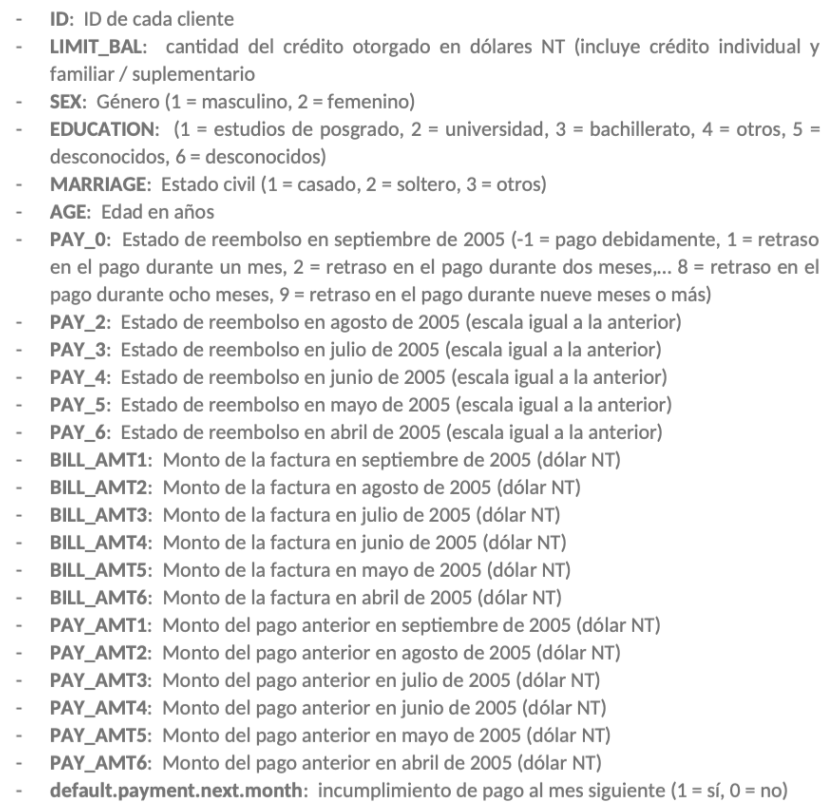
\includegraphics[scale=0.5]{Images/1}
\end{figure}
Estadísticas de los datos luego de la limpieza: 
\begin{figure}[H]
	\centering
	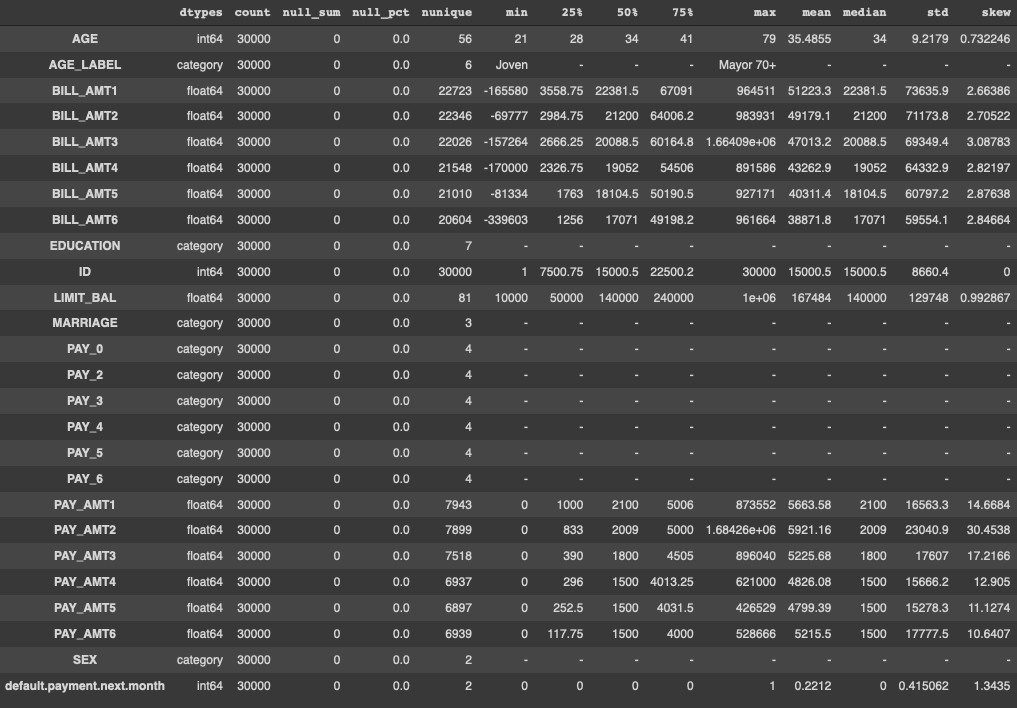
\includegraphics[scale=0.4]{Images/2}
\end{figure}

\subsection{Descripciones individuales}
\begin{cajita}
	Todas las operaciones de limpieza fueron ejecutadas automáticamente por medio de QuickDA: duplicados, nulos y tipo de varibles. 
\end{cajita}

\begin{figure}[H]
	\centering
	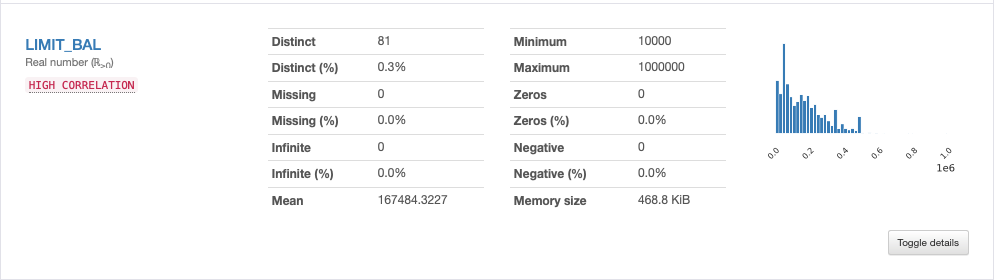
\includegraphics[scale=0.4]{Images/3}
\end{figure}
\begin{figure}[H]
	\centering
	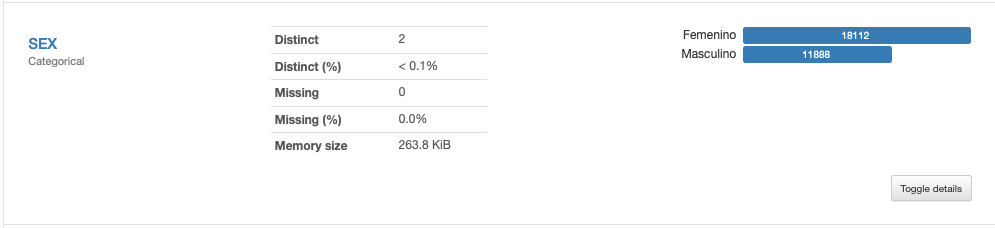
\includegraphics[scale=0.4]{Images/4}
\end{figure}
\begin{figure}[H]
	\centering
	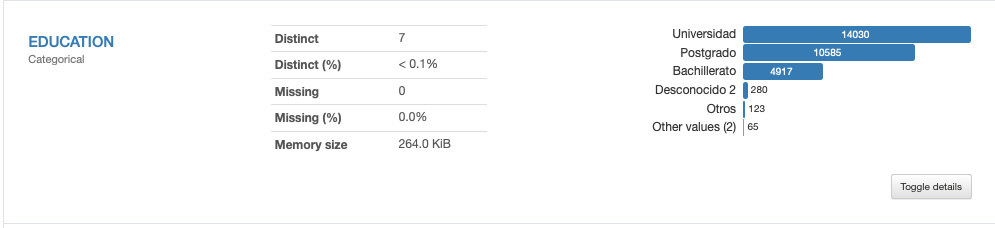
\includegraphics[scale=0.4]{Images/5}
\end{figure}
\begin{figure}[H]
	\centering
	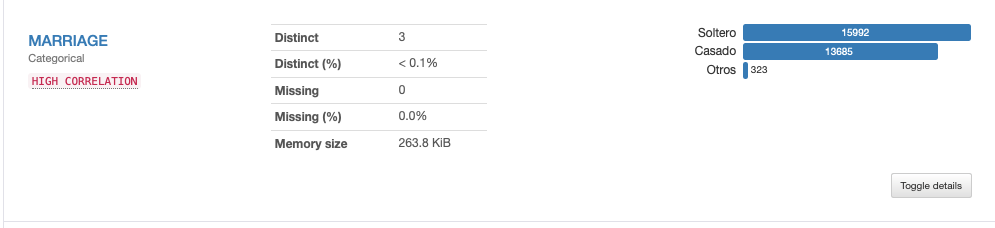
\includegraphics[scale=0.4]{Images/6}
\end{figure}
\begin{figure}[H]
	\centering
	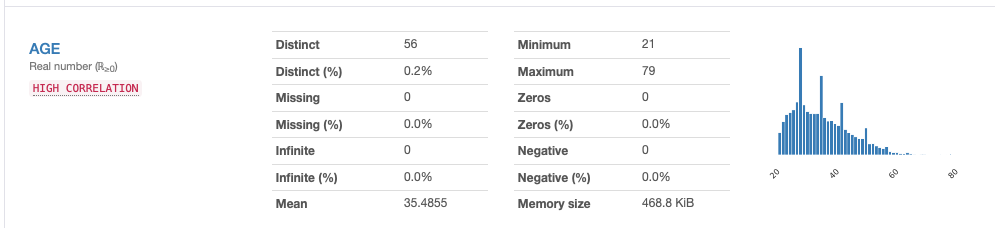
\includegraphics[scale=0.4]{Images/7}
\end{figure}\begin{figure}[H]
\centering
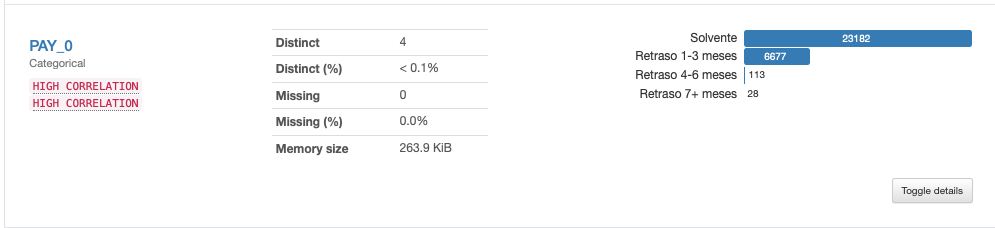
\includegraphics[scale=0.4]{Images/8}
\end{figure}\begin{figure}[H]
\centering
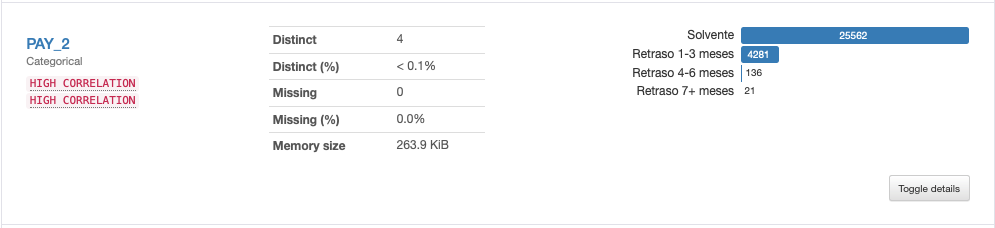
\includegraphics[scale=0.4]{Images/9}
\end{figure}\begin{figure}[H]
\centering
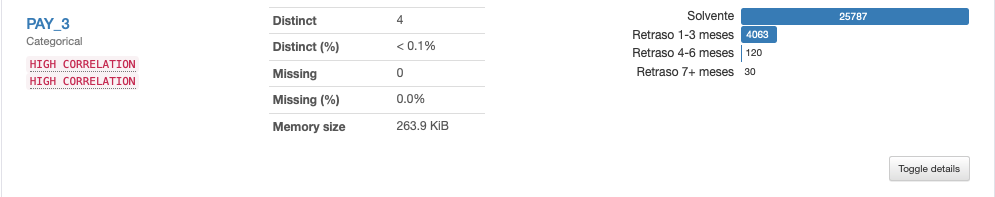
\includegraphics[scale=0.4]{Images/10}
\end{figure}
\begin{figure}[H]
	\centering
	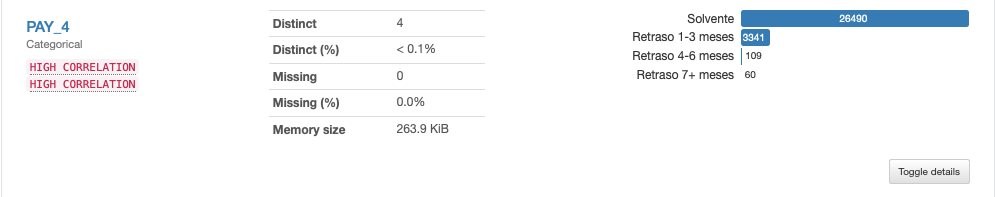
\includegraphics[scale=0.4]{Images/11}
\end{figure}
\begin{figure}[H]
	\centering
	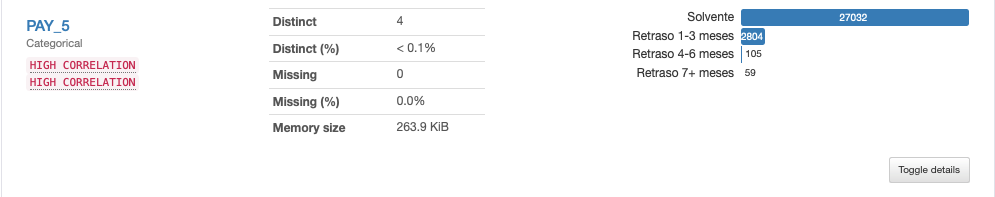
\includegraphics[scale=0.4]{Images/12}
\end{figure}
\begin{figure}[H]
	\centering
	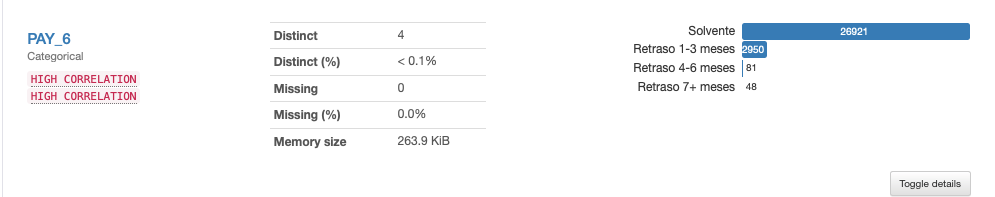
\includegraphics[scale=0.4]{Images/13}
\end{figure}
\begin{figure}[H]
	\centering
	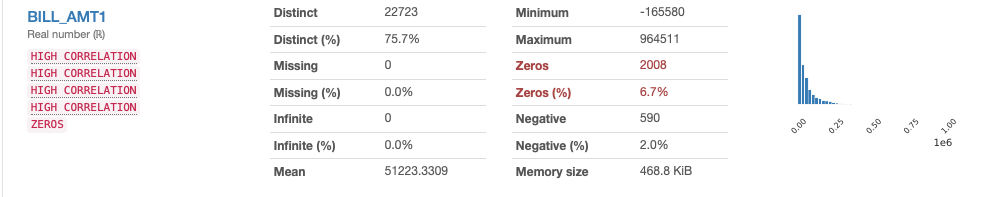
\includegraphics[scale=0.4]{Images/14}
\end{figure}
\begin{figure}[H]
	\centering
	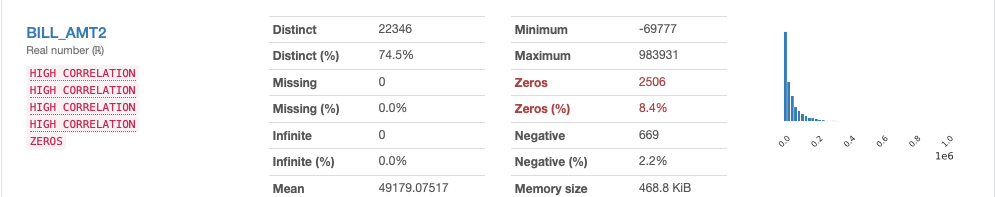
\includegraphics[scale=0.4]{Images/15}
\end{figure}
\begin{figure}[H]
	\centering
	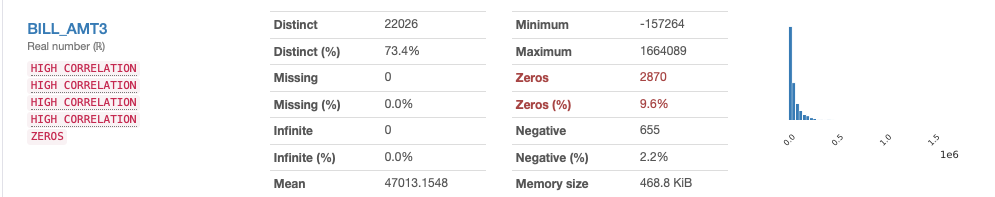
\includegraphics[scale=0.4]{Images/16}
\end{figure}
\begin{figure}[H]
	\centering
	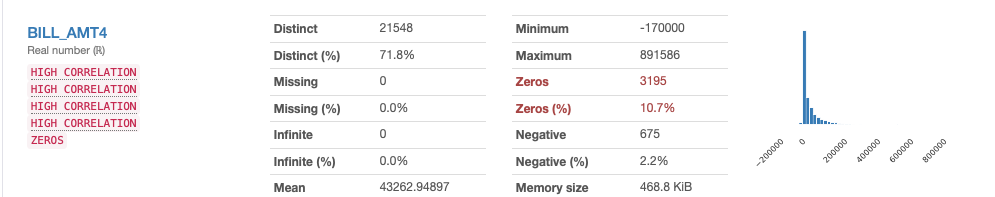
\includegraphics[scale=0.4]{Images/17}
\end{figure}
\begin{figure}[H]
	\centering
	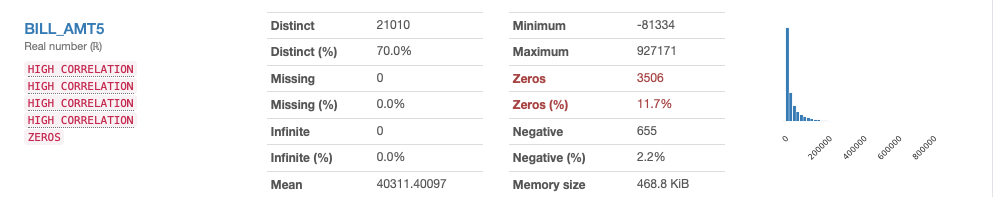
\includegraphics[scale=0.4]{Images/18}
\end{figure}
\begin{figure}[H]
	\centering
	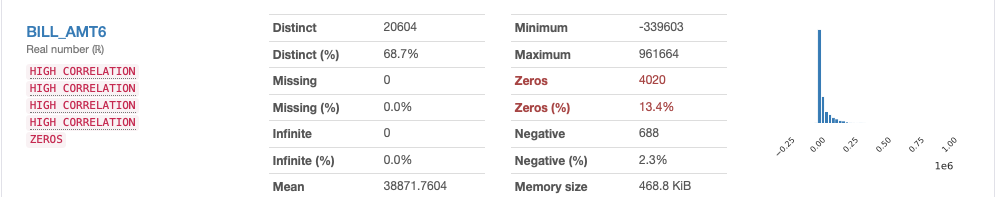
\includegraphics[scale=0.4]{Images/19}
\end{figure}
\begin{figure}[H]
	\centering
	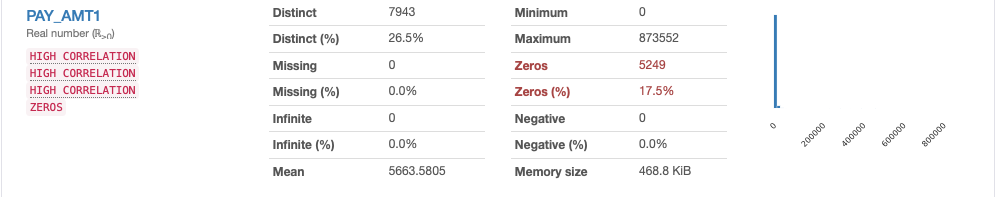
\includegraphics[scale=0.4]{Images/20}
\end{figure}
\begin{figure}[H]
	\centering
	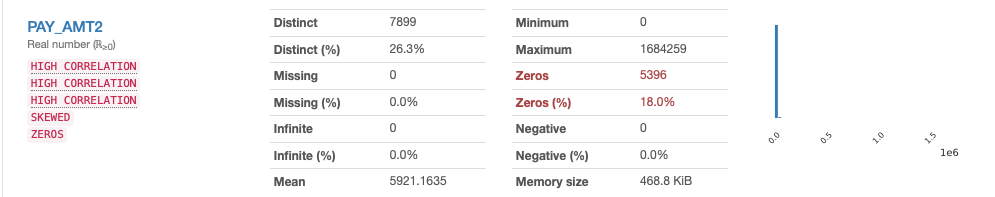
\includegraphics[scale=0.4]{Images/21}
\end{figure}
\begin{figure}[H]
	\centering
	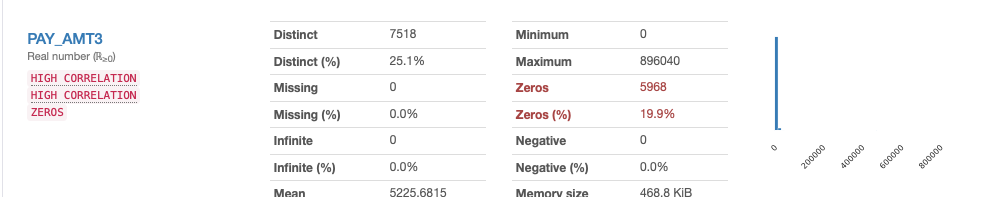
\includegraphics[scale=0.4]{Images/22}
\end{figure}\begin{figure}[H]
\centering
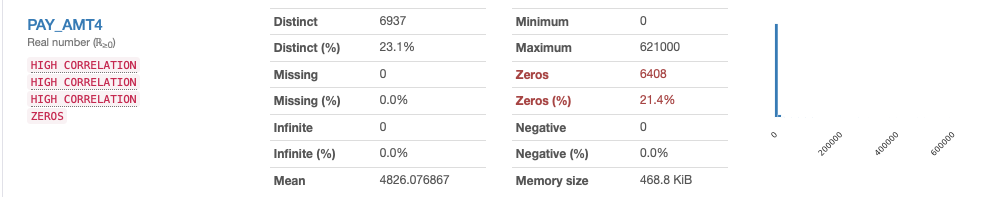
\includegraphics[scale=0.4]{Images/23}
\end{figure}
\begin{figure}[H]
	\centering
	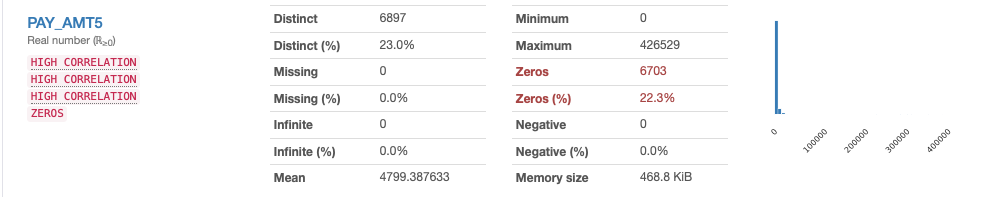
\includegraphics[scale=0.4]{Images/24}
\end{figure}
\begin{figure}[H]
	\centering
	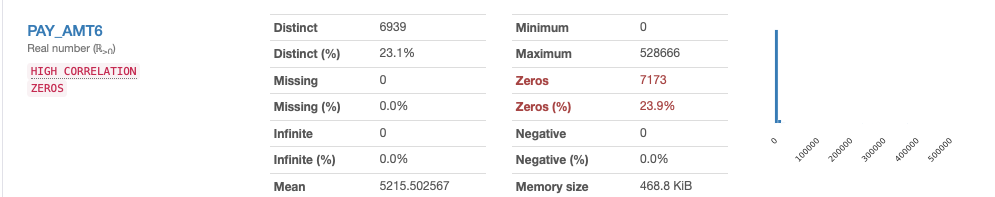
\includegraphics[scale=0.4]{Images/25}
\end{figure}
\begin{figure}[H]
	\centering
	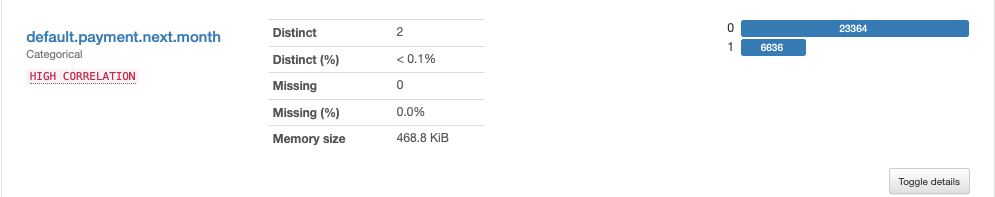
\includegraphics[scale=0.4]{Images/26}
\end{figure}
\begin{figure}[H]
	\centering
	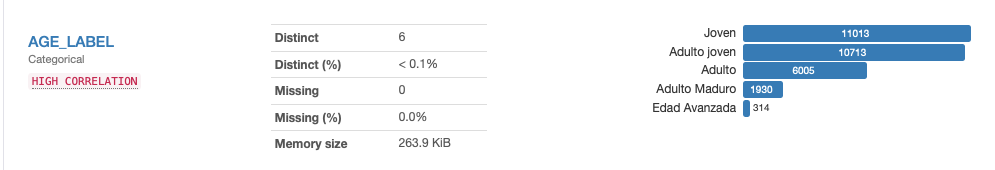
\includegraphics[scale=0.4]{Images/27}
\end{figure}


\section{Análisis exploratorio}

El análisis exploratorio (explicado) puede ser encontrado  al final de este archivo.
\section{Hallazgos y conclusiones}

\subsection{Resumen hallazgos}
El resumen de hallazgos puede ser encontrado en la sección de «análisis específicos» del \textit{Jupyter Notebook} adjuntado. 

\subsection{Conclusiones}

\begin{enumerate}
	\item Se determinaron nuevas subvariables para varias variables ya preexistentes con el propósito de dar una mejor perspectiva a los datos; como en el caso de la edad, para tener una distribución por edades. 
	\item  Se cruzaron varias variables para determinar sus relaciones y su implicación directa con la cantidad de crédito otorgado; para entender a mayor profundidad y dar una perspectiva intuitiva acerca de los datos. 
	\item Se comprobó el estado de los datos para determinar datos atípicos, duplicados y datos nulos; los cuales ayudarán a obtener mejores resultados en el modelo. 
\end{enumerate}


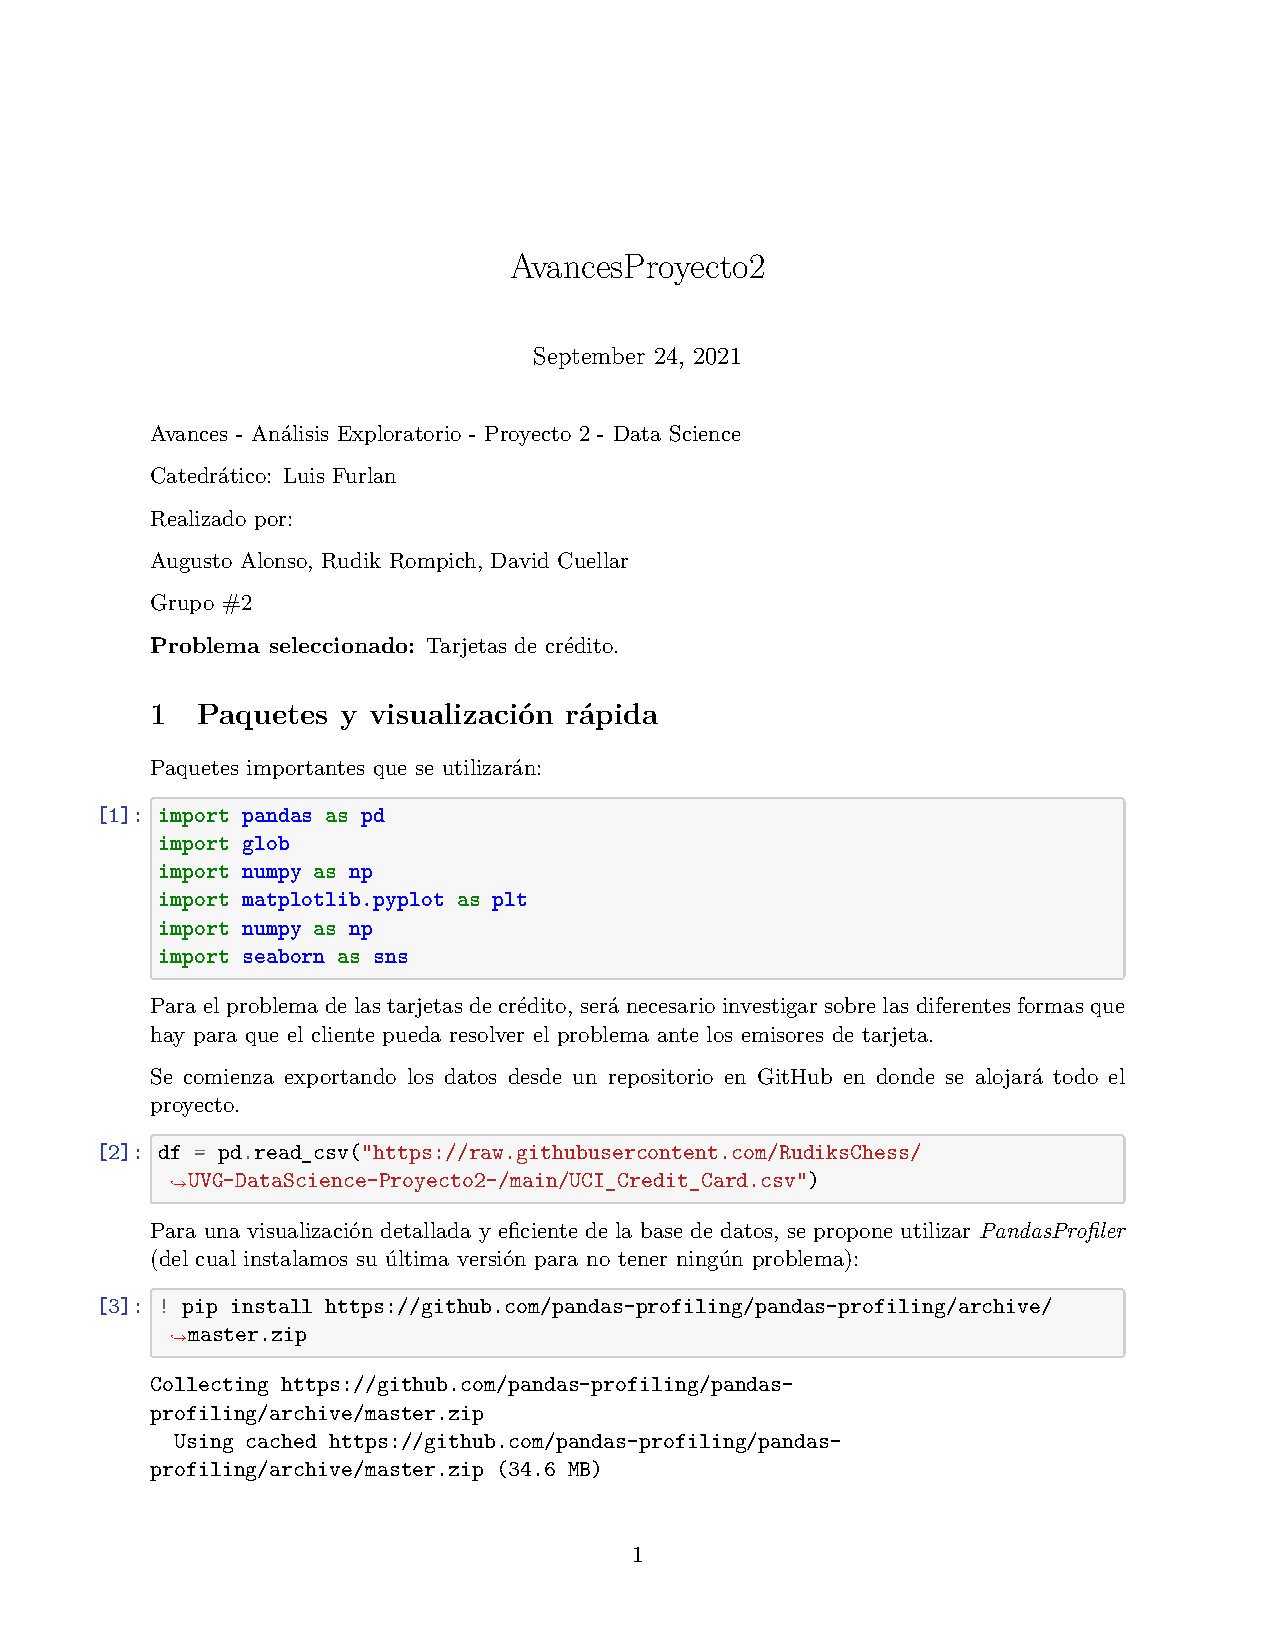
\includepdf[pages=-]{Images/AE.pdf}

%---------------------------
\bibliographystyle{apa}
\bibliography{referencias.bib}

\end{document}